% =============================================================================
% Overleaf template for algorithm documentation
%
% How to use:
%   1. Replace \ProjectName and \AlgorithmName below.
%   2. Fill the Input / Output tables in Section 1.
%   3. Replace the stage labels in the TikZ diagram with your pipeline.
%   4. Keep one notation table and use those symbols consistently.
%   5. Put the high-level loop in the algorithm float, and detailed math in
%      Section 5. Do not duplicate the same formula in three places.
%   6. Add one worked example with real numbers and a limitations section.
%
% Compile with pdfLaTeX on Overleaf. The template uses only standard packages.
% =============================================================================

\documentclass[11pt]{article}

\usepackage[margin=1in]{geometry}
\usepackage{amsmath,amssymb,amsthm,mathtools}
\usepackage{booktabs,tabularx,array}
\usepackage{graphicx}
\usepackage{xcolor}
\usepackage{tikz}
\usetikzlibrary{arrows.meta,positioning,calc,fit,backgrounds}
\usepackage{algorithm}
\usepackage{algpseudocode}
\usepackage[hidelinks]{hyperref}
\usepackage{cleveref}

% -----------------------------------------------------------------------------
% Paper metadata
% -----------------------------------------------------------------------------
\newcommand{\ProjectName}{Project Name}
\newcommand{\AlgorithmName}{Algorithm Name}
\newcommand{\ph}[1]{\textcolor{gray}{#1}}   % placeholder text

\newtheorem{definition}{Definition}
\newtheorem{assumption}{Assumption}

\DeclareMathOperator*{\argmax}{arg\,max}
\DeclareMathOperator*{\argmin}{arg\,min}
\newcommand{\R}{\mathbb{R}}
\newcommand{\E}{\mathbb{E}}
\newcommand{\indicator}[1]{\mathbf{1}\!\left[#1\right]}
\newcommand{\proc}[1]{\text{\textsc{#1}}}
\newcommand{\vect}[1]{\mathbf{#1}}
\newcommand{\set}[1]{\mathcal{#1}}

\title{\textbf{\ProjectName}\\[2pt]
\large Algorithm Documentation: \AlgorithmName}
\author{\ph{Author Name}\\\ph{Affiliation}}
\date{\ph{Date or version}}

\begin{document}
\maketitle

\begin{abstract}
\ph{One paragraph: what problem the algorithm solves, what its inputs and outputs
are, what is novel, and what evidence supports the claim. State the evaluation
boundary explicitly. Avoid claiming a calibrated score unless it was calibrated.}
\end{abstract}

\tableofcontents

% =============================================================================
\section{Problem definition}
% =============================================================================

\subsection{Input and output}

\begin{table}[h]
\centering
\small
\begin{tabularx}{\textwidth}{@{}l l X@{}}
\toprule
\textbf{Input} & \textbf{Domain} & \textbf{Description} \\
\midrule
$I$ & $\R^{H \times W \times 3}$ & \ph{Input image, color space, value range.} \\
$q$ & $\Sigma^\ast$ & \ph{Search description or task specification.} \\
$\theta$ & $\Theta$ & \ph{Configuration: budgets, thresholds, weights.} \\
\ph{optional} & \ph{type} & \ph{Injected model, cache, or prior.} \\
\bottomrule
\end{tabularx}
\caption{Inputs. Keep the domain and units explicit.}
\label{tab:inputs}
\end{table}

\begin{table}[h]
\centering
\small
\begin{tabularx}{\textwidth}{@{}l l X@{}}
\toprule
\textbf{Output} & \textbf{Domain} & \textbf{Description} \\
\midrule
$\set{R}$ & $(\set{B} \times \R)^{K}$ & \ph{Ranked regions with scores.} \\
$\set{T}$ & tree & \ph{Search tree, statistics, and expansion order.} \\
$\tau$ & sequence & \ph{Allocation trace: selected path and reward per step.} \\
$u$ & counters & \ph{Actual calls, tokens, cache hits, and cost.} \\
$s$ & finite set & \ph{Stop reason.} \\
\bottomrule
\end{tabularx}
\caption{Outputs. Separate the model output from diagnostics and artifacts.}
\label{tab:outputs}
\end{table}

\subsection{Scope and non-goals}

\begin{itemize}
  \item \textbf{In scope.} \ph{What the algorithm is responsible for.}
  \item \textbf{Out of scope.} \ph{What a downstream component handles.}
  \item \textbf{Evidence boundary.} \ph{What the metric measures and what it does
  not measure. For example: IoU is a localization proxy, not answer accuracy.}
\end{itemize}

% =============================================================================
\section{Notation}
% =============================================================================

\begin{table}[h]
\centering
\small
\begin{tabularx}{\textwidth}{@{}l X@{}}
\toprule
\textbf{Symbol} & \textbf{Meaning} \\
\midrule
$v \in \set{V}$ & Search-tree node (region). \\
$v_0$ & Root node, usually the whole image. \\
$\set{C}(v)$ & Active children of $v$. \\
$n_v$ & Completed evaluations backed up through $v$. \\
$R_v$ & Sum of raw rewards backed up through $v$. \\
$Q_v$ & Empirical mean reward, $Q_v = R_v / n_v$. \\
$U_v$ & Exploration bonus. \\
$C_v$ & Forecast remaining cost below $v$. \\
$r_v$ & Raw reward returned by one complete evaluation of $v$. \\
$\set{A}(v)$ & Admissible branches at $v$. \\
$\set{K}$ & Checked candidates in one region evaluation. \\
$\set{K}^{+}$ & Verified candidates, $\set{K}^{+} \subseteq \set{K}$. \\
$K_{\max}$ & Count cap at which the count reward saturates. \\
$\lambda$ & Cost-penalty weight. \\
$T_{\mathrm{ref}}$ & Cost normalization constant, in seconds. \\
\bottomrule
\end{tabularx}
\caption{Notation. Add every symbol that appears in an equation or algorithm.}
\label{tab:notation}
\end{table}

% =============================================================================
\section{Algorithm at a glance}
% =============================================================================

\begin{figure}[t]
\centering
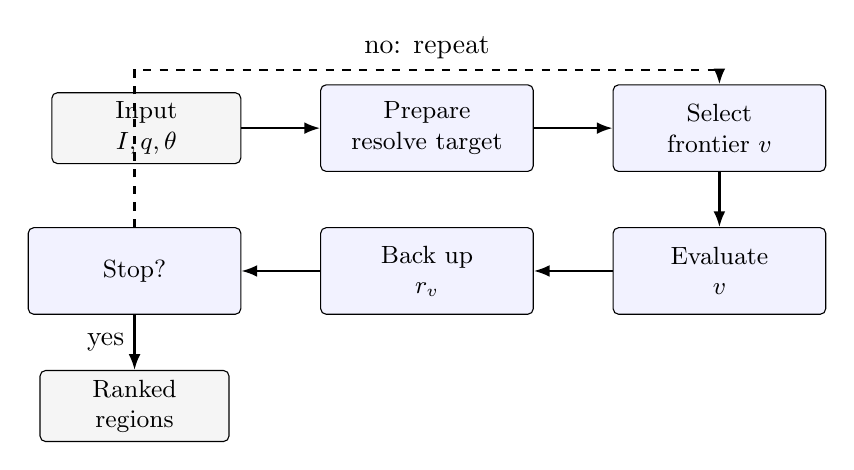
\begin{tikzpicture}[
  node distance=7mm and 10mm,
  stage/.style={draw, rounded corners=2pt, align=center,
                minimum width=2.7cm, minimum height=1.1cm,
                fill=blue!5, font=\small},
  data/.style={draw, rounded corners=2pt, align=center,
               minimum width=2.4cm, minimum height=0.9cm,
               fill=gray!8, font=\small},
  arrow/.style={-{Latex[length=2mm]}, thick},
  loop/.style={-{Latex[length=2mm]}, thick, dashed}
]
  \node[data] (in) {Input\\$I, q, \theta$};
  \node[stage, right=of in] (prep) {Prepare\\resolve target};
  \node[stage, right=of prep] (select) {Select\\frontier $v$};
  \node[stage, below=of select] (eval) {Evaluate\\$v$};
  \node[stage, left=of eval] (backup) {Back up\\$r_v$};
  \node[stage, left=of backup] (stop) {Stop?};
  \node[data, below=of stop] (out) {Ranked\\regions};

  \draw[arrow] (in) -- (prep);
  \draw[arrow] (prep) -- (select);
  \draw[arrow] (select) -- (eval);
  \draw[arrow] (eval) -- (backup);
  \draw[arrow] (backup) -- (stop);
  \draw[arrow] (stop) -- node[left] {yes} (out);
  \draw[loop] (stop.north) -- ++(0,2.0)
    -| node[pos=0.25, above] {no: repeat} (select.north);
\end{tikzpicture}
\caption{End-to-end control flow. Replace the five stage labels with your own
pipeline. The dashed edge is the bounded search loop.}
\label{fig:pipeline}
\end{figure}

\subsection{Step-by-step view}

\begin{table}[h]
\centering
\small
\begin{tabularx}{\textwidth}{@{}c l X X@{}}
\toprule
\textbf{Step} & \textbf{Operation} & \textbf{What changes} & \textbf{Evidence to save} \\
\midrule
0 & Prepare & \ph{Validate request, load models, resolve target.} & \ph{Config, model IDs, resolved prompt.} \\
1 & Initialize & \ph{Create root and first children.} & \ph{Root statistics and split decision.} \\
2 & Select & \ph{Choose one frontier with Eq.~\eqref{eq:selection}.} & \ph{Path, terms, excluded branches.} \\
3 & Evaluate & \ph{Detect, verify, and score one region.} & \ph{Exact inputs, raw replies, components.} \\
4 & Back up & \ph{Update $n_v$ and $R_v$ on the selected path.} & \ph{Before/after statistics.} \\
5 & Expand & \ph{Split the evaluated node, or mark it exhausted.} & \ph{Children, geometry checks, fallback.} \\
6 & Stop & \ph{Apply the stopping rule and rank all evidence.} & \ph{Stop reason, ranked output, usage.} \\
\bottomrule
\end{tabularx}
\caption{One iteration as a sequence of independently auditable operations.}
\label{tab:steps}
\end{table}

% =============================================================================
\section{High-level pseudocode}
% =============================================================================

\begin{algorithm}[t]
\caption{Bounded recursive search}
\label{alg:search}
\begin{algorithmic}[1]
\Require image $I$, query $q$, configuration $\theta$
\Ensure ranked regions $\set{R}$, tree $\set{T}$, trace $\tau$, usage $u$
\State $s \gets \proc{Prepare}(I,q,\theta)$
\State $\set{T} \gets \proc{NewTree}(\proc{Root}(I))$
\State $\proc{Expand}(\set{T}.\text{root}, s)$
\While{not $\proc{Stop}(\set{T},s)$}
  \State $P \gets \proc{SelectPath}(\set{T},s)$
  \Comment{Eq.~\eqref{eq:selection}}
  \State $v \gets \text{last}(P)$
  \State $e \gets \proc{Evaluate}(v,s)$
  \State $\proc{Backup}(P,e.r)$
  \State $\proc{Expand}(v,s)$
\EndWhile
\State $\set{R} \gets \proc{Rank}(\set{T})$
\State \Return $\set{R}, \set{T}, \tau, u$
\end{algorithmic}
\end{algorithm}

\paragraph{How to read the pseudocode.}
The algorithm above deliberately hides model internals in \textsc{Evaluate}.
Put the model-specific work in a separate helper or equation, not in the main
loop. The main loop should expose only: the selected branch, the returned reward,
the backup, and the stopping rule.

% =============================================================================
\section{Mathematical formulation}
% =============================================================================

\subsection{Search state}

Let $\set{T} = (\set{V}, \set{E})$ be the tree. For a node $v \in \set{V}$,
let $n_v$ be the number of complete evaluations backed up through $v$, and
$R_v$ the sum of their raw rewards. Define

\begin{equation}
  Q_v = \frac{R_v}{n_v}, \qquad n_v > 0,
  \label{eq:quality}
\end{equation}
and $Q_v = 0$ for an unvisited node. The backed-up reward is the same at every
level; cost is not subtracted from $R_v$.

\subsection{Selection rule}

For an expanded node $v$ with admissible children $\set{A}(v)$,

\begin{equation}
  a^\star
  = \argmax_{a \in \set{A}(v)}
    \left[
      Q_a
      + c \sqrt{\frac{\ln(n_v + 1)}{n_a}}
      - \lambda \frac{C_a}{T_{\mathrm{ref}}}
    \right],
  \label{eq:selection}
\end{equation}
where the second term is zero when $n_a = 0$, and the third term is omitted for
plain UCT. Ties are broken by the lowest node ID.

The remaining-cost forecast is recursive:
\begin{equation}
  C_v =
  \begin{cases}
    \max\bigl(0, \hat{c}(v)\bigr), & \set{C}(v) = \varnothing, \\[4pt]
    \displaystyle
    \sum_{u \in \set{C}(v)}
      \frac{n_u + 1/|\set{C}(v)|}
           {\sum_{w \in \set{C}(v)} n_w + 1}
      \, C_u, & \text{otherwise},
  \end{cases}
  \label{eq:cost}
\end{equation}
where $\hat{c}(v)$ estimates the uncached detection, verification, and split
work at the frontier.

\subsection{Reward}

For one evaluated region, let $\set{K}$ be the checked candidates. A candidate
is \emph{verified} when
\begin{equation}
  \text{verified}(k)
  = \indicator{\text{answer}_k = \text{Yes}}
    \indicator{\text{score}_k \ge \tau_{\mathrm{accept}}}.
\end{equation}
For the verified set $\set{K}^{+}$ define
\begin{align}
  q^\star &= \max_{k \in \set{K}} \{\text{score}_k : \text{answer}_k \ne \text{No}\}, \\
  \bar{s} &= \frac{1}{|\set{K}^{+}|}
             \sum_{k \in \set{K}^{+}} s_k, \\
  \kappa &= \frac{\min(|\set{K}^{+}|, K_{\max})}{K_{\max}}, \\
  \bar{\iota} &= \frac{1}{\binom{|\set{K}^{+}|}{2}}
             \sum_{\{i,j\} \subseteq \set{K}^{+}}
             \operatorname{IoU}(b_i,b_j), \\
  \delta &= 1 - \bar{\iota},
\end{align}
where $s_k$ is detector confidence, $K_{\max}$ is the count cap, and $b_k$ is a box.
The region reward is
\begin{equation}
  r_v =
  \begin{cases}
    \displaystyle
    \frac{
      w_q q^\star + w_s \bar{s} + w_\kappa \kappa + w_\delta \delta
    }{
      w_q + w_s + w_\kappa + w_\delta
    }, & \set{K}^{+} \ne \varnothing, \\[8pt]
    0, & \text{otherwise}.
  \end{cases}
  \label{eq:reward}
\end{equation}
If $|\set{K}^{+}| = 1$, set $\bar{\iota} = 0$ and $\delta = 1$. If no candidate exists, $q^\star = 0$.

\subsection{Stopping rule}

The search stops when any condition in
\begin{equation}
  \text{stop} \in
  \{\text{exhausted}, \text{api-budget}, \text{local-budget},
    \text{iterations}, \text{match}, \text{error}\}
\end{equation}
holds. A partial evaluation interrupted by a budget must not update $n_v$ or
$R_v$.

% =============================================================================
\section{Worked example}
% =============================================================================

\paragraph{Example: \texttt{0411\_q01}.}
\ph{Replace this paragraph and table with one real run. State why the case was
chosen; do not select it as a success story without saying it was selected after
the run.}

\begin{table}[h]
\centering
\small
\begin{tabularx}{\textwidth}{@{}l X@{}}
\toprule
Question & What color is the shirt worn by the person operating the TV camera on the upper balcony? \\
Resolved target & The person operating the TV camera \\
Image size & $4269 \times 2846$ \\
Annotated target & $[2342, 1810, 2418, 1923]$ \\
Top-1 / best IoU & $0.9574$ / $0.9574$ \\
Verification path & Per-candidate context/detail sheets, early stop at first \texttt{Yes} \\
Calls / stop reason & 8 local image generations; \texttt{local\_budget} \\
\bottomrule
\end{tabularx}
\caption{A compact record of one successful localization. Ground truth was used
only after inference for inspection.}
\label{tab:example}
\end{table}

\paragraph{What happened.}
\ph{Give three to five concrete steps with numbers: first-pass box, recursive
child, score components, and final rank. Explain the mechanism, not just the
metric.}

\begin{figure}[h]
\centering
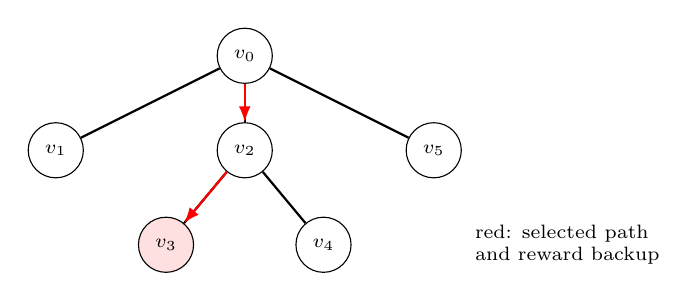
\begin{tikzpicture}[
  circ/.style={circle, draw, minimum size=7mm, font=\scriptsize},
  path/.style={-{Latex[length=2mm]}, thick, red},
  edge/.style={thick}
]
  \node[circ] (r) at (0,0) {$v_0$};
  \node[circ] (a) at (-2.4,-1.2) {$v_1$};
  \node[circ] (b) at (0,-1.2) {$v_2$};
  \node[circ, fill=red!12] (c) at (-1.0,-2.4) {$v_3$};
  \node[circ] (d) at (1.0,-2.4) {$v_4$};
  \node[circ] (e) at (2.4,-1.2) {$v_5$};
  \draw[edge] (r) -- (a);
  \draw[edge] (r) -- (b);
  \draw[edge] (r) -- (e);
  \draw[edge] (b) -- (c);
  \draw[edge] (b) -- (d);
  \draw[path] (r) -- (b);
  \draw[path] (b) -- (c);
  \node[align=left, font=\scriptsize, anchor=west] at (2.8,-2.4)
    {red: selected path\\and reward backup};
\end{tikzpicture}
\caption{A tree snapshot. Show the selected path, the evaluated leaf, and the
nodes that received a backup. Replace this with a snapshot from your own run.}
\label{fig:tree}
\end{figure}

% =============================================================================
\section{Operations and cost model}
% =============================================================================

\begin{table}[h]
\centering
\small
\begin{tabularx}{\textwidth}{@{}l l X@{}}
\toprule
\textbf{Stage} & \textbf{Cost unit} & \textbf{What is cached or bounded} \\
\midrule
Prepare & model load, text generation & \ph{Resolver called once; models loaded lazily.} \\
Detect & detector forward pass & \ph{Per-node detection cache.} \\
Verify & verifier generation & \ph{Per-region or per-candidate batch; hard budget.} \\
Split & feature encoder + clustering & \ph{One split per node; depth and pixel limits.} \\
Rank & sort & \ph{No model calls.} \\
\bottomrule
\end{tabularx}
\caption{Account for every operation separately. Do not collapse local
generations, detector calls, and HTTP calls into one ``cost'' number.}
\label{tab:cost}
\end{table}

The loop performs at most $N_{\max}$ evaluations, where $N_{\max}$ is the
smallest applicable budget,
\begin{equation}
  N_{\max} = \min\left(
    \text{max-iterations},
    \; \text{api-budget},
    \; \text{local-budget}
  \right),
\end{equation}
with an unlimited budget treated as $+\infty$. A complete evaluation costs one
detector pass plus one or more verifier calls; a split costs one feature
encoding, one SLIC sweep over the candidate counts, and one clustering pass. In
this implementation, the local budget counts verifier generations, and each
evaluation adds one detector pass and at most one split.

% =============================================================================
\section{Failure modes and limitations}
% =============================================================================

\begin{itemize}
  \item \textbf{Detector miss.} \ph{The search can only split regions it has.}
  \item \textbf{Verifier error.} \ph{Malformed output must be uncertainty, not a
  zero reward.}
  \item \textbf{Reward bias.} \ph{List terms that can dominate or saturate.}
  \item \textbf{Budget truncation.} \ph{The result is the best evidence so far,
  not a proof of global optimality.}
  \item \textbf{Measurement boundary.} \ph{IoU, top-1, and answer accuracy are
  different claims.}
\end{itemize}

% =============================================================================
\section{Reproducibility checklist}
% =============================================================================

\begin{enumerate}
  \item Record the exact model IDs, revisions, and device.
  \item Record the full configuration, including defaults that were not changed.
  \item Save the resolved target phrase and every verifier input.
  \item Save raw verifier responses, not only parsed scores.
  \item Report every stop reason and every incomplete step.
  \item Separate inference inputs from post-run ground-truth inspection.
  \item Freeze the code and data hashes before reading evaluation labels.
\end{enumerate}

% =============================================================================
% References
% =============================================================================
\begin{thebibliography}{9}
\bibitem{uct}
\ph{Author. \emph{Title}. Venue, Year.}
\bibitem{agentuct}
\ph{Author. \emph{Title}. Venue, Year.}
\end{thebibliography}

\end{document}
